\section{Odraz míčku}
\label{sec:odraz-micku}

Samotný odraz je pro tuto práci nejdůležitější. Tedy bude probrán velmi
podrobně. Důležitým předpokladem je, že $\speed{1}$ a $\spin{1}$ jsou hodnoty přímo
před odrazem. Díky tomuto předpokladu nemusíme uvažovat let míčku
popsaný v \myref{sekci}{sec:let-micku} ani jeho letové vlastnosti.

Problém je i tak stále velmi komplexní, protože na odraz má vliv hned několik
proměnných. Ty společně s charakteristikou celé odrazové periody budou popsány v
této sekci.

Obecně se všechny proměnné v tomto problému dají rozřadit do tří kategorií:

\begin{description}
 \item[Nezávislé] Pro tuto práci to jsou: $\speed{1}$, $\spin{1}$ a $\angle{1}$.
 \item[Závislé] Analogicky se jedná o: $\speed{2}$, $\spin{2}$ a $\angle{2}$.
 \item[Kontrolované] Jde především o materiálové konstanty:
  vertikální/horizontální koeficient restituce ($e_{x/y}$), koeficient smýkavého
 tření ($\mu$), poloměr ($R$), koeficient momentu hybnosti ($\alpha$),
 vzdálenost geometrického středu od působení normálové síly ($D$).
\end{description}

Závislé a nezávislé proměnné jsou znázorněné na \myref{obrázku}{fig:odraz-micku}.
Nezávislé jsou proměnné před odrazem a na nich závisí proměnné po odraze.
Kontrolované proměnné na \myref{obrázku}{fig:odraz-micku} nejsou, ale stále je
důležité je uvést pro replikovatelnost výsledků. Také budou z pravidla přebírány
z odborné literatury, a tedy nebudou v této práci měřené.

\begin{figure}[htbp]
 \centering
 \documentclass{article}
\usepackage{tikz}
\usepackage{xcolor}
\usepackage{mathtools}

\definecolor{darkgreen}{rgb}{0.0,0.5,0.0}
\begin{document}

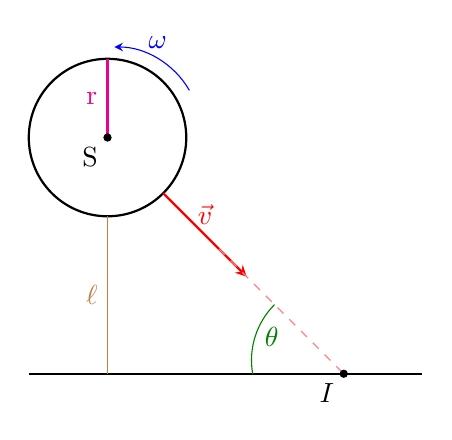
\begin{tikzpicture}
	%ball
	\draw[thick] (0,0) circle (1);
	%radius
	\draw[magenta,thick] (0,0) --node[midway,left] {r}++ (0,1);
	\node[fill=black,circle,inner sep=0pt, minimum size=3pt](s) at (0,0) {};
	%center
	\node[below left](slabel) {S};

	%speed
	\draw[red,thick,-stealth](-45:1) --node[above] {$\vec{v}$}++ (-45:1.5);
	\draw[red!50,dashed](-45:2) -- (-45:4.3);

	%graund
	\draw[thick] (-1,-3) -- (4,-3);

	%vercial length
	\draw[brown] (0,-1) --node[left] {$\ell$}++ (0,-2);

	%angle
	\node[fill=black,circle,inner sep=0pt, minimum size=3pt](naraz) at (3,-3)
	{};
	\node[below left] at (naraz) {$I$};

	\draw[darkgreen] (-45:3) arc[
			start angle = 135,
			end angle = 190,
			radius = 1,
		] node[midway,right] {$\theta$};

	%angular velocity
	\draw[blue,-stealth] (30:1.2) arc(30:90:1.1) node[midway,above] {$\omega$};
\end{tikzpicture}
\end{document}



 \caption{Síly a veličiny působící na míček při odrazu}
 \label{fig:odraz-micku}
\end{figure}

\subsection{Koeficienty restituce}
\label{ssec:koeficienty-restituce}
Koeficient restituce ($e$) vyjadřuje jak moc je odraz elastický, kolik energie
se v něm ztratí. Perfektně elastický odraz s $e=1$ tedy znamená, že při odrazu
nedojde k disipaci žádné energie. Taková odraz je ovšem v praktických podmínkách
nereálný. Hodnoty $e$ jsou v rozmezí $0 \leq e \geq 1$ kde $e=0$ znamená ztrátu
veškeré energie a už nedochází k žádnému odrazu.
\autocite{ahmadImpactModelsCoefficient2016,CoefficientRestitutionFormula}

Pro náš případ bude důležité rozdělit koeficient restituce na tečný a
vertikální ($e_{x/y}$). Tečnou komponentu budeme uvažovat v bodě, nebo ploše,
kde míček přichází do kontaktu s odrazovou plochou.

Jak bude popsáno v
\myref{podsekci}{ssec:treni-po-dobu-odrazu} na míček v průběhu kontaktu působí
tření, které není po celou dobu ve stejném směru. Pro tento případ by byl
nejpřesnější koeficient restituce odvozený z práce, kterou míček a odrazová
plocha vykonají za dobu odrazu. Pro jednoduchost bude $e$ zaveden podle Newtona
následovně\autocite{ahmadImpactModelsCoefficient2016}:
$e =  \sped{1}/\sped{2}$.

Rozdělení $e$ na jeho vertikální a tečnou komponentu můžeme vidět na
rovnicích \ref{eq:COR} a \ref{eq:CORR}. Na rozdíl od $e_y$ není definice $e_x$ intuitivní. Aby
byla tato definice logicky motivovaná je třeba vrátit se k obecné defnici z
předchozího odstavce.

\begin{align} 
 \label{eq:COR}
  e_y &= \frac{\sped{y2}}{\sped{y1}} \\
  \label{eq:CORR}
 e_x &= -\frac{(\sped{x2}-R\spn{\omega_2})}{{(\sped{x1}}-R\spn{1})}
\end{align}

\subsubsection{Lineární a úhlová rychlost}
\label{ssec:linearni-a-uhlova-rychlost}

Obecně by koeficient restituce měl být poměr lineární rychlosti před a po
odrazu. V našem případě musíme vzít v potaz, že míček má úhlovou rychlost, která
se s tou lineární sčítá.\autocite{WhyPeopleEdge2017,TangentialVelocityFormula}
Proto ji musíme odečíst abychom získali jen lineární složku rychlosti.

\begin{figure}[htbp]
 \centering
 \begin{tikzpicture}
 %circle
 \draw[thick] (-1,0) arc[
  start angle=180,
  end angle=360,
  radius=1
  ];
%vertical
 \draw[velcol, -stealth] (0,-1) --node[left] {$\speed{y}$} (0,-2);
%horizontal plus tangential
 \draw[velcol,-stealth] (0,-1) --node[below]
  {$\speed{x}\textcolor{black}{+}\speed{t}$} (1.5,-1);

 %only tangential
 \draw[velcol,-stealth] (0.75,-0.7) --node[right]
  {$\speed{t}\textcolor{black}{=R}\spin{}$}
  (1.3,0);

 








\end{tikzpicture}


 \caption{Tečná, horizontální a vertikální komponenta rychlosti}
 \label{fig:tecna-rychlost}
\end{figure}

Jak můžeme vidět na \myref{obrázku}{fig:tecna-rychlost}, tečná a horizontální
složka míří stejným směrem,\footnote{Rovnoběžné jsou tyto složky jen pro póly
míčku, ale mají stejné znaménko, pro všechny body na obvodu (pro $\sped{x} > 0$ a $ \spn{}
<0$). My koeficient restituce počítáme pro bod v kontaktu s odrazovou plochou
tedy zmíněné výpočty
platí.\autocite{crossBounceSpinningBall2005,hierrezueloSlidingRollingPhysics1995} Jinak by bylo zapotřebí započítat odchylku
$\speed{x}$ a $\speed{t}$.} tedy horizontální získáme jako
$\sped{x}-R\spn{}$. Tento výraz můžeme vidět
v \myref{rovnici}{eq:CORR}.

\subsection{Moment hybnosti}
\label{ssec:moment-hybnosti}
Moment hybnosti je rotační ekvivalent hybnosti a udává se k nějaké ose. V našem
případě tato osa prochází středem míčku a v \myref{obrázku}{fig:diagram} si ji
můžeme představit jako kolmou na celý obrázek. Úhlová rychlost také je udávána k
této ose.

Moment hybnosti definujme jako\autocite{MomentInertiaa}:
\[
 \vec{L}=I\spin{}
\]
Kde pro náš případ se moment setrvačnosti ($I$) rovná $\alpha m R^2$. Koeficient
momentu hybnosti ($\alpha$) závisí na tom jaký míček si vybereme. \texttt{Jestli
zbude čas rád bych napsal apendix o tom jak integrovat v kouli jakoukoliv funkci
hustoty a podle toho získal koeficient momentu hybnosti.} Pro pevný plný míček
$\aplha=2/5$, pro dutou kouli $\alpha=2/3$\autocite{crossGripslipBehaviorBouncing2002,MomentInertiaa}. Míček na stolní tennis je natolik
tenký, že jeho koeficient momentu hybnosti aproximujeme na $2/3$.

\subsubsection{Moment hybnosti během odrazu}
\label{ssec:moment-hybnosti-behem-odrazu}

V průběhu odrazu se mění úhlová rychlost a s ní i moment hybnosti. Kromě $\alpha$
může mít na změnu $L$ vliv \textcolor{frcol}{$\vec{F}$}, a
\textcolor{brown}{$\vec{N}$}. 

U normálové síly (\textcolor{brown}{$\vec{N}$}) je jednoduché nahlédnout, v
jakém případě ovlivňuje moment hybnosti. Z \myref{obrázku}{fig:odraz-micku} je
zřejmé, že když normálová síla působí přímo pod geometrickým středem
míčku\footnote{Neboli $D=0$} tak nikterak nepřispívá do úhlového momentu. 

U síly třecí je to poněkud složitější. Ta když směřuje proti směru rotace tak
zmenšuje úhlovou rychlost a s ní i moment hybnosti. Jak bude popsáno v
\myref{podsekci}{ssec:treni-odraz} tření může směřovat i ve směru úhlové rychlosti.
Proto záleží na orientaci \textcolor{frcol}{$\vec{F}$}.

Horizontální vzdálenost normálové síly a geometrického středu máme již zavedenou
a to jako $D$. Proto $D\textcolor{brown}{N}$ je moment hybnosti během odrazu s
nulovým třením.\autocite{hierrezueloSlidingRollingPhysics1995} Když doplníme vliv tření získáme: $D\textcolor{brown}{N} \pm
R\textcolor{frcol}{F} = I\spn{}$. Kde samozřejmě znaménko záleží na směru
tření.\autocite{crossGripslipBehaviorBouncing2002,Cross_2018}

\subsection{Tření po dobu odrazu}
\label{ssec:treni-odraz}
Abychom mohli opodstatnit myšlenky v této podsekci musíme si zavést dynamické
tření obecně. Poté bude jednoduché nahlédnout do tření po dobu odrazu.

\subsubsection{Dynamické tření}
\label{sssec:dynamicke-treni}

Směr dynamického tření je vždy opačný k relativní rychlosti dvou těles, které
mezi sebou tření tvoří. Matematicky dynamické tření vyjádříme
jako\autocite{WhatDynamicFriction,hierrezueloSlidingRollingPhysics1995}:
\[
 \textcolor{frcol}{F}=\mu \textcolor{brown}{N}
\]
Kde důležitou konstantou je koeficient dynamického tření ($\mu$), které je
empiricky měřeno. $\mu$ je materiálová konstanta pro oba z povrchů přítomných při
tření. Dále budou materiály vybírány tak aby jejich $\mu$ bylo již naměřeno.

\subsubsection{Směr tření při odrazu}
\label{sssec:smer-treni-pri-odrazu}

Pro popsání tření při odrazu předpokládejme, že $\spn{1}=0$. Tento předpoklad
platí také pro \myref{obrázek}{fig:treni}. Jakmile míček přichází do kontaktu s
odrazovou plochou začíná na něj působit tření. To směřuje proti směru $\sped{x}$
a tedy se $\sped{x}$ zmenšuje. Druhý méně jasný efekt je změna momentu hybnosti.
Tření zpomaluje jen tu část míčku v kontaktu s druhým povrchem, horní polovina
se ovšem pohybuje stále stejně rychle tedy dochází k přeměně lineární rychlosti
na tu
úhlovou.\autocite{hierrezueloSlidingRollingPhysics1995,crossBounceSpinningBall2005}
Tento efekt je znázorněn v části \textbf{a)} \myref{obrázku}{fig:treni}.

Zmenšování $\sped{x}$ a zvětšování $\spn{}$ probíhá jen do chvíle kdy
$\sped{x}=R\spn{}$. Poté ještě chvíli pokračuje v takzvaném \uv{gripu} (ten
můžeme vidět v části \textbf{b)}. V \uv{gripu} je míček pouze díky statickému
tření. Jakmile moment hybnosti přeroste statické tření míček přechází do
\uv{rolování}.\autocite{hierrezueloSlidingRollingPhysics1995,crossGripslipBehaviorBouncing2002}

Rolování, které můžeme vidět v části \textbf{c)}, je nejméně intuitivní ze všech
částí odrazu. Směr tření se v něm totiž otočí a působí po směru $\sped{x}$. Jak již
bylo řečeno tření působí proti směru relativního pohybu dvou povrchů. Ve chvíli
kdy $\sped{x} < R\spn{}$ tak spodek míčku po povrchu podkluzuje. Tedy relativní
pohyb dvou povrchů je ve směru rotace. Tření v tomto případě působí proti směru
$\spn{}$ a po směru $\sped{x}$.\autocite{crossGripslipBehaviorBouncing2002}

Když se míček při rolování neodrazí od podložky může se stát, že díky tření se
přes \uv{grip} zase míček dostane do \uv{slidování}, které již bylo popsáno a je znázorněno v
sekci \textbf{a)} \myref{obrázku}{fig:treni}, a tedy že $\sped{x} > R\spn{}$.
Jestliže odraz tvrdá dostatečně dlouho, cyklů  
\begin{inparaenum}
\item sliding
\item grip
\item roling
\item grip
\end{inparaenum}
se stihne vystřídat hned několik.\autocite{crossGripslipBehaviorBouncing2002}

\begin{figure}[htbp]
 \centering
 \begin{tikzpicture}
 %ground
 \draw[thick] (0,0) -- (9,0);

 %first ball
 \draw[thick] (0.5,0) arc[
  start angle =230,
  end angle = -50,
  radius = 1
  ];

 %friction
 \draw[thick,-stealth,frcol] (1,-0.2) --node[below,frcol] {$\vec{F}$} (2,-0.2);
 %label
 \node[thick,black] at (0.5,2.5) {\textbf{a)} $\sped{x}>R\spn{}$}
 %angular momentum
 \draw[thick,spcol] (0.1,1) arc[
	 start angle = 180,
	 end angle = 120,
	 radius = 0.9] node[midway,left, above=5pt] {$\spin{}$}

 %second ball
 \draw[thick] (3.5,0) arc[
  start angle = 210,
  end angle = -30,
  radius =1
  ]

%friction
\draw[thick, -stealth, frcol] (4,-0.2) --node[below, frcol] {$\vec{F}$}
 (5,-0.2);

\node[thick,black] at (4,2.5) {\textbf{b)} $\sped{x}>R\spn{}$}


  %third ball
  \draw[thick] (7,0)  arc[
  start angle =230,
  end angle = -50,
  radius = 1
  ];

\draw[thick, stealth-, frcol] (7,-0.2) --node[below, frcol] {$\vec{F}$}
 (8,-0.2);

\node[thick,black] at (7.5,2.5) {\textbf{c)} $\sped{x}<R\spn{}$}

 


\end{tikzpicture}


 \caption{Směr tření po dobu odrazu}
 \label{fig:treni}
\end{figure}


\subsection{Triviální případy}
\label{ssec:trivialni-pripady}



